\documentclass[12pt]{article}
\usepackage[authoryear,round]{natbib}
\usepackage{amsmath,amssymb,amsfonts}
\usepackage{algorithmic}
\usepackage{graphicx}
\usepackage{textcomp}
\usepackage{xcolor}
\usepackage{booktabs}
\usepackage{multirow}
\usepackage{url}
\usepackage{hyperref}
\usepackage[margin=1in]{geometry}
\setlength{\parskip}{0.15em}
\setcounter{topnumber}{2}
\renewcommand{\topfraction}{0.9}
\renewcommand{\textfraction}{0.07}
\renewcommand{\floatpagefraction}{0.8}
\makeatletter
\renewcommand{\@biblabel}[1]{}
\makeatother
\setlength{\bibsep}{0pt}

\begin{document}

\title{CarbonEdge: A Real-Time Multi-Cloud Cost and Carbon Emission Optimization Framework with Transformer-Based Forecasting}

\author{
\normalsize Shah Abulkalam Ahteshamuddin Kunjenashin$^{1,*}$, Dr. Prafullata K. Auradkar$^{1}$\\[4pt]
\small $^{1}$Department of Computer Science and Engineering, PES University, Bengaluru, India\\
\small $^{*}$Corresponding author(s) E-mail(s): \small {shah.official1011@gmail.com}, {prafullata.auradkar@pes.edu}\\
}
\date{}

\maketitle

\begin{abstract}
Cloud users usually choose virtual machines by cost and performance, while instance-level environmental impact remains opaque across providers. This paper presents CarbonEdge, a real-time multi-cloud decision framework that jointly optimizes monetary cost and carbon emissions across Amazon Web Services (AWS), Microsoft Azure, and Google Cloud Platform (GCP). CarbonEdge combines live pricing feeds with regional carbon intensity and uses an interpretable instance-level model based on vCPU, memory, utilization, and idle-power fraction. Candidate instances are ranked with a Pareto-style multi-objective strategy and returned as three actionable recommendations: lowest cost, lowest emissions, and best trade-off. For proactive planning, a Temporal Fusion Transformer (TFT) is trained on multi-year carbon-intensity data across provider-region groups to generate seven-day probabilistic forecasts. Results show large region-driven differences for the same workload and demonstrate that substantial emission reduction is possible with moderate cost premiums. The framework is implemented as a deployable FastAPI and Next.js system for practical sustainability-aware cloud selection.
\end{abstract}

\noindent\textbf{Keywords:} multi-cloud optimization; carbon emissions; sustainability; Pareto optimization; temporal fusion transformer; cloud computing

\section{Introduction}
Cloud adoption continues to accelerate, with public cloud spending projected to exceed \$800 billion by 2025 \citep{b1}. In practice, resource selection is still dominated by cost and performance metrics, while environmental impact is rarely visible at the instance level. Although cloud vendors provide sustainability dashboards \citep{b2,b3,b4}, those tools are generally provider-specific and not designed for real-time cross-provider, instance-level decision making.

This gap is important because the same compute workload can produce significantly different emissions across regions due to electricity-grid variation. Users therefore need a practical mechanism to compare cost and carbon jointly before deployment.

CarbonEdge addresses this need with four contributions:
\begin{enumerate}
    \item An interpretable instance-level carbon model that combines power estimation and regional carbon intensity.
    \item A real-time multi-cloud comparison pipeline across AWS, Azure, and GCP.
    \item A multi-objective recommendation layer that outputs cheapest, greenest, and balanced options.
    \item A forecasting module (TFT) that supports short-horizon, uncertainty-aware planning.
\end{enumerate}

\section{Related Work}
Prior work on cloud optimization has focused primarily on cost, including right-sizing and pricing-aware scheduling. Sustainability-focused work has shown the value of carbon-aware scheduling at data-center scale \citep{b3,b4}, but practical instance-level decision support across providers remains limited.

Carbon estimation methods typically combine power models and grid carbon data \citep{b9,b10,b11}. Multi-objective techniques such as Pareto analysis and NSGA-II are well established in cloud optimization \citep{b13,b14}, though real-time integration of cost and emissions in user-facing tools is less common. For forecasting, TFT offers strong multi-horizon capability and interpretable attention \citep{b15,b16}.

Recent studies reinforce the need for operational tools: simulation-driven multi-cloud cost-carbon frameworks \citep{b17} and pricing comparison studies \citep{b18} are informative but do not provide a deployable real-time platform. Infrastructure-level optimization frameworks \citep{b19} are valuable but target operators rather than end users.

\section{System Overview}
CarbonEdge uses a three-tier architecture: frontend dashboard, backend API/engine, and external data sources.

\begin{figure}[!t]
\centering
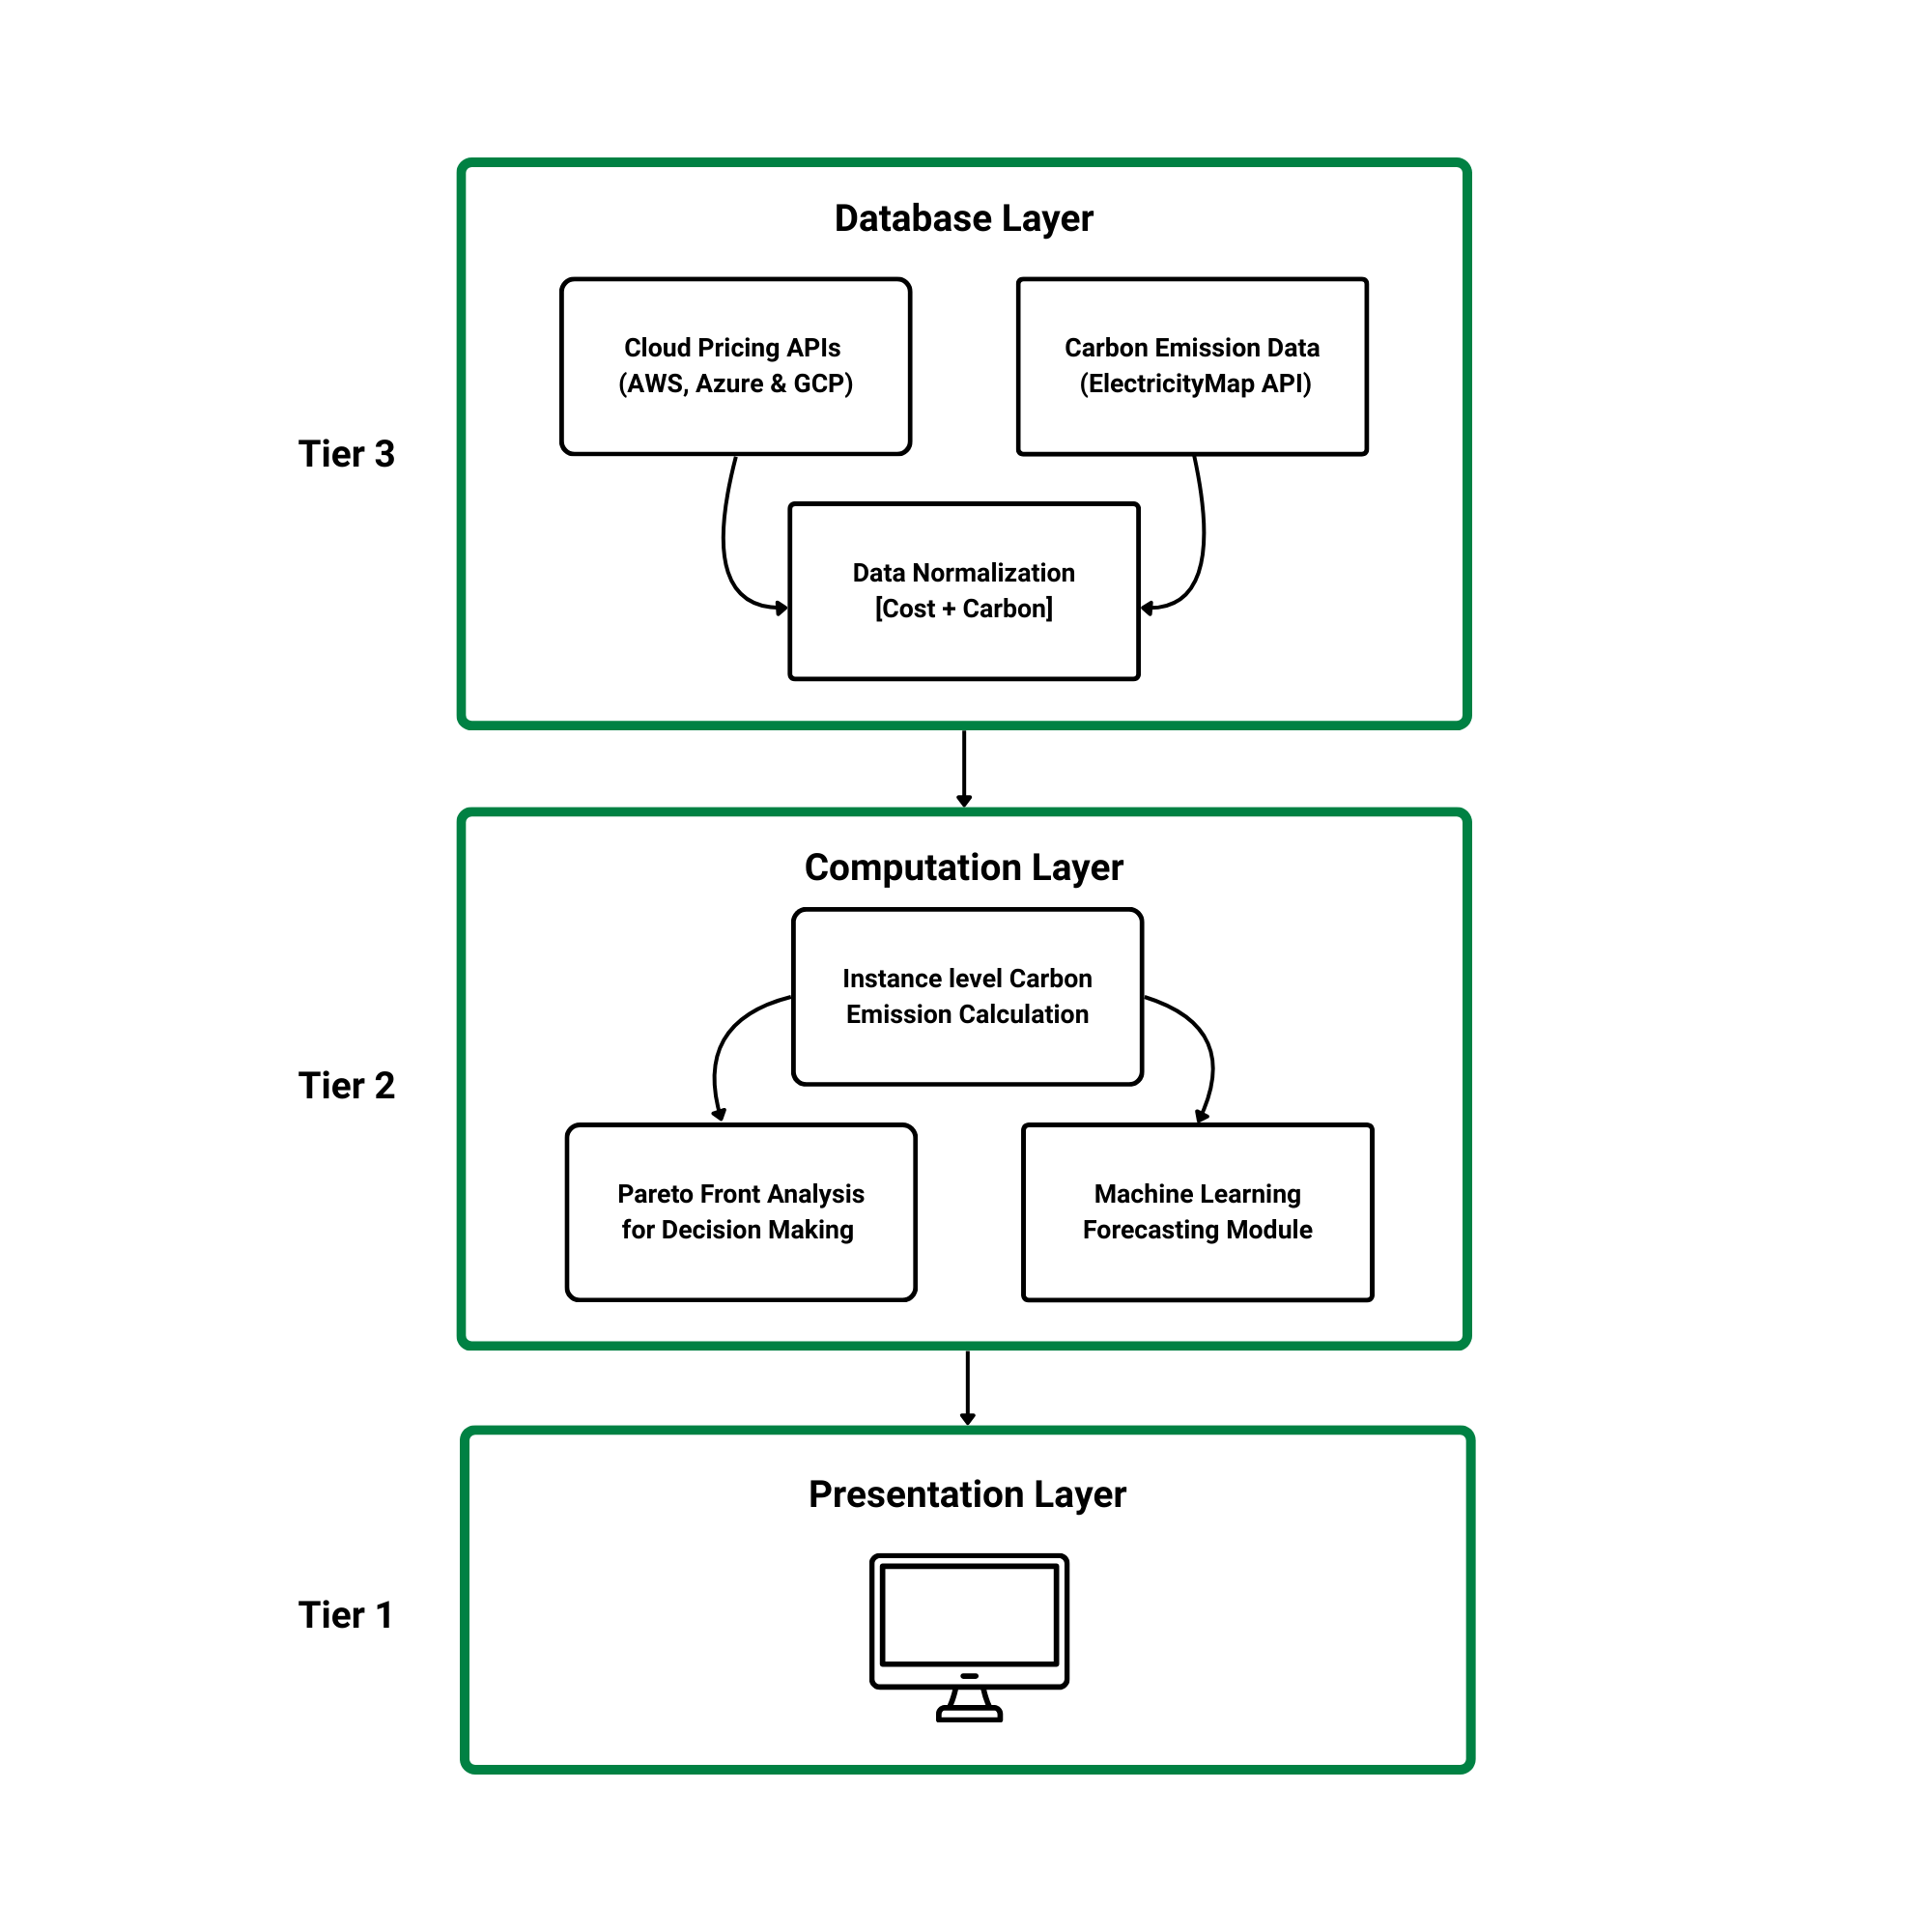
\includegraphics[width=0.72\textwidth]{3tier}
\caption{CarbonEdge system architecture.}
\label{fig:architecture}
\end{figure}

\subsection{Pipeline}
\begin{enumerate}
    \item User submits workload constraints (vCPU, RAM, storage, utilization) and providers.
    \item Backend retrieves candidate instances and prices from AWS, Azure, and GCP sources.
    \item Regions are mapped to carbon zones and real-time carbon intensity is fetched.
    \item Instance-level emissions are computed.
    \item Pareto-style ranking generates three recommendations.
    \item Optional seven-day forecasts are attached for planning support.
\end{enumerate}

\section{Methodology}
\subsection{Instance-Level Carbon Estimation}
Maximum power is estimated from CPU and memory terms:
\begin{equation}
P_{\text{max}} = v\,P_{\text{cpu}} + m\,P_{\text{mem}}
\end{equation}

Idle power is modeled as a fraction of peak power:
\begin{equation}
P_{\text{idle}} = \alpha\,P_{\text{max}}
\end{equation}

Power at utilization $u$:
\begin{equation}
P_{\text{actual}} = P_{\text{max}}\,(\alpha + u(1-\alpha))
\end{equation}

Hourly emissions are then:
\begin{equation}
\text{CO}_{2}^{\text{instance}} = \frac{(vP_{\text{cpu}} + mP_{\text{mem}})(\alpha + u(1-\alpha))}{1000}\times CI
\label{eq:co2}
\end{equation}
where $CI$ is regional carbon intensity from ElectricityMap \citep{b9}.

Parameter values used in this work are $P_{\text{cpu}}=15$ W, $P_{\text{mem}}=1.5$ W, and $\alpha=0.35$, aligned with prior power-modeling literature \citep{b10,b11}. Table~\ref{tab:params} summarizes these parameters and their justifications.

\begin{table}[!t]
\centering
\caption{Carbon estimation model parameters.}
\label{tab:params}
\small
\begin{tabular}{lcl}
\toprule
\textbf{Symbol} & \textbf{Value} & \textbf{Justification} \\
\midrule
$P_{\text{cpu}}$ & 15.0~W & SPECpower benchmarks; \citet{b10} \\
$P_{\text{mem}}$ & 1.5~W  & DDR4/DDR5 power models; \citet{b11} \\
$\alpha$          & 0.35   & Typical idle-to-peak server power ratio \\
$u$               & 0--1   & User-specified utilization factor \\
$CI$              & varies & Real-time from ElectricityMap \citep{b9} \\
\bottomrule
\end{tabular}
\end{table}

These values are empirically grounded: 15~W/vCPU covers the typical 10--20~W range for modern server cores, 1.5~W/GB reflects DDR4/DDR5 DIMM power, and $\alpha=0.35$ matches commonly reported idle-to-peak behavior.

\subsection{Cost-Carbon Multi-Objective Ranking}
For each candidate instance $i$, cost $c_i$ and emission $e_i$ are min-max normalized:
\begin{equation}
\hat{c}_i = \frac{c_i-c_{\min}}{c_{\max}-c_{\min}}, \quad
\hat{e}_i = \frac{e_i-e_{\min}}{e_{\max}-e_{\min}}
\end{equation}

A combined score is computed:
\begin{equation}
S_i = \hat{c}_i + \hat{e}_i
\end{equation}

Returned recommendations are:
\begin{itemize}
    \item cheapest: $\arg\min c_i$
    \item lowest emissions: $\arg\min e_i$
    \item best trade-off: $\arg\min S_i$
\end{itemize}

\subsection{TFT Forecasting Model}
CarbonEdge uses the Temporal Fusion Transformer \citep{b15} with a 30-day encoder and 7-day prediction horizon on daily aggregated carbon-intensity series. Calendar covariates (day-of-week, month, week-of-year, weekend flag, quarter) and provider-region group identifiers are included as known inputs. The model is trained with quantile loss across seven quantiles $q \in \{0.02, 0.1, 0.25, 0.5, 0.75, 0.9, 0.98\}$, with the median serving as the point forecast and P10--P90 forming the 80\% prediction interval. Table~\ref{tab:hyperparams} lists the key hyperparameters.

\begin{table}[!t]
\centering
\caption{TFT model hyperparameters.}
\label{tab:hyperparams}
\small
\begin{tabular}{lr}
\toprule
\textbf{Hyperparameter} & \textbf{Value} \\
\midrule
Encoder / prediction length (days) & 30 / 7 \\
Batch size & 64 \\
Max epochs (with early stopping) & 50 \\
Learning rate & $1\times10^{-3}$ \\
Hidden size / attention heads & 32 / 2 \\
Dropout / gradient clip & 0.1 / 0.1 \\
Train/val split (temporal) & 85/15 \\
\bottomrule
\end{tabular}
\end{table}

The split is temporal (not random); series are normalized per group using a GroupNormalizer with softplus transformation.

\section{Implementation}
The backend is implemented in FastAPI with provider-specific pricing adapters and a carbon-intensity integration module. Region-to-zone mapping is handled through YAML configurations. The frontend (Next.js) exposes two workflows: decision mode (instance recommendations) and forecast mode (regional trend exploration).

The forecasting service uses a cached singleton pattern to reduce repeated inference overhead for frequent regional queries.

\section{Evaluation}

\subsection{Dataset Statistics}
The carbon intensity dataset comprises hourly readings from the ElectricityMap API over approximately three years (January 2022 to early 2025). After daily aggregation and quality filtering (minimum 365 days per group), the dataset contains over 60 provider-region groups with more than 1,100 time steps per group, yielding 392 held-out validation forecast points.

\subsection{Carbon Emission Comparison Across Regions}
Table~\ref{tab:carbon_comparison} presents estimated CO\textsubscript{2} emissions for a representative 4~vCPU, 16~GB workload at 50\% utilization across selected regions.

\begin{table}[!t]
\centering
\caption{CO\textsubscript{2} emissions (g/hr) for 4 vCPU, 16 GB RAM at 50\% utilization across selected regions.}
\label{tab:carbon_comparison}
\small
\begin{tabular}{llrr}
\toprule
\textbf{Provider} & \textbf{Region} & \textbf{CI (gCO\textsubscript{2}/kWh)} & \textbf{CO\textsubscript{2} (g/hr)} \\
\midrule
AWS & eu-west-3 (Paris) & $\sim$60 & $\sim$3.56 \\
Azure & francecentral & $\sim$60 & $\sim$3.56 \\
GCP & europe-north1 (Finland) & $\sim$90 & $\sim$5.35 \\
AWS & ca-central-1 (Canada) & $\sim$120 & $\sim$7.13 \\
Azure & uksouth (London) & $\sim$250 & $\sim$14.85 \\
AWS & us-east-1 (Virginia) & $\sim$400 & $\sim$23.76 \\
GCP & asia-east1 (Taiwan) & $\sim$550 & $\sim$32.67 \\
AWS & ap-south-1 (Mumbai) & $\sim$650 & $\sim$38.61 \\
Azure & southafricanorth & $\sim$750 & $\sim$44.55 \\
\bottomrule
\end{tabular}
\end{table}

The same workload produces approximately 3.56~gCO\textsubscript{2}/hr in France (nuclear-dominated grid, CI~$\approx$~60~gCO\textsubscript{2}/kWh) compared to 44.55~gCO\textsubscript{2}/hr in South Africa (coal-dominated grid, CI~$\approx$~750~gCO\textsubscript{2}/kWh)---a factor of more than 12$\times$. Region selection therefore dominates emission outcomes even when instance class and utilization are held fixed.

\subsection{Utilization Sensitivity Analysis}
Table~\ref{tab:utilization_sensitivity} reports CO\textsubscript{2} values at three utilization levels for the same workload using a fixed reference carbon intensity of 400~gCO\textsubscript{2}eq/kWh, with $P_{\text{cpu}}=15$~W, $P_{\text{mem}}=1.5$~W, and $\alpha=0.35$.

\begin{table}[!t]
\centering
\caption{Sensitivity of estimated CO\textsubscript{2} to utilization (4 vCPU, 16 GB RAM, CI = 400~gCO\textsubscript{2}eq/kWh).}
\label{tab:utilization_sensitivity}
\small
\begin{tabular}{lr}
\toprule
\textbf{Utilization} & \textbf{CO\textsubscript{2} (g/hr)} \\
\midrule
25\% & 17.22 \\
50\% & 22.68 \\
75\% & 28.14 \\
\bottomrule
\end{tabular}
\end{table}

Emissions increase approximately linearly with utilization, confirming that utilization-aware scheduling can materially reduce carbon impact for variable workloads.

\subsection{Multi-Objective Optimization Results}
Table~\ref{tab:pareto_results} illustrates the three-way recommendation output for a sample 4~vCPU, 16~GB, 100~GB storage workload.

\begin{table}[!t]
\centering
\caption{Multi-objective recommendation comparison for 4 vCPU, 16 GB workload.}
\label{tab:pareto_results}
\small
\begin{tabular}{lllrr}
\toprule
\textbf{Recommendation} & \textbf{Provider} & \textbf{Instance} & \textbf{\$/hr} & \textbf{gCO\textsubscript{2}/hr} \\
\midrule
Cheapest & GCP & e2-standard-4 & 0.1008 & 23.76 \\
Lowest CO\textsubscript{2} & AWS & m5.xlarge & 0.1920 & 3.56 \\
Eco-Optimized & Azure & Standard\_D4s\_v3 & 0.1440 & 7.13 \\
\bottomrule
\end{tabular}
\end{table}

The cheapest option (GCP \texttt{e2-standard-4} in \texttt{us-central1}) costs \$0.1008/hr but produces 23.76~gCO\textsubscript{2}/hr. The lowest-CO\textsubscript{2} option (AWS \texttt{m5.xlarge} in \texttt{eu-west-3}) reduces emissions to 3.56~gCO\textsubscript{2}/hr at \$0.1920/hr. The eco-optimized recommendation (Azure \texttt{Standard\_D4s\_v3} in \texttt{canadacentral}) provides a balanced trade-off at \$0.1440/hr and 7.13~gCO\textsubscript{2}/hr, representing a 70\% emission reduction over the cheapest option for a 43\% cost premium.

\begin{figure}[!t]
\centering
\includegraphics[width=0.72\textwidth]{pareto}
\caption{Pareto-front scatter plot showing cost vs.\ CO\textsubscript{2} emissions for candidate instances. The eco-optimized instance (star marker) lies on the Pareto front, balancing both objectives.}
\label{fig:pareto}
\end{figure}

\subsection{TFT Forecast Evaluation}
The TFT model is evaluated on the held-out validation set (last 15\% of temporal data). Table~\ref{tab:forecast_metrics} reports aggregated metrics across all region groups.

\begin{table}[!t]
\centering
\caption{TFT forecasting accuracy metrics (aggregated across all regions, 7-day horizon).}
\label{tab:forecast_metrics}
\small
\begin{tabular}{lr}
\toprule
\textbf{Metric} & \textbf{Value} \\
\midrule
Mean Absolute Error (MAE) & 36.20 \\
Root Mean Square Error (RMSE) & 53.04 \\
Mean Absolute Percentage Error (MAPE) & 17.74\% \\
80\% Prediction interval coverage & 65.05\% \\
Model parameters & $\sim$94.5K \\
\bottomrule
\multicolumn{2}{l}{\footnotesize Metrics on held-out validation split (392 forecast points).} \\
\end{tabular}
\end{table}

The TFT captures regional differences and temporal patterns. Regions with stable energy mixes (e.g., France, Canada) exhibit narrower prediction intervals, while volatile grids (e.g., Germany, UK) show wider uncertainty bands. An MAE of 36.20 and MAPE of 17.74\% across 60+ heterogeneous provider-region groups is sufficient for trend-aware planning. The 80\% prediction interval coverage of 65.05\% indicates mild under-calibration, but uncertainty bands remain informative for classifying regional trends as increasing, stable, or decreasing.

\begin{figure}[!t]
\centering
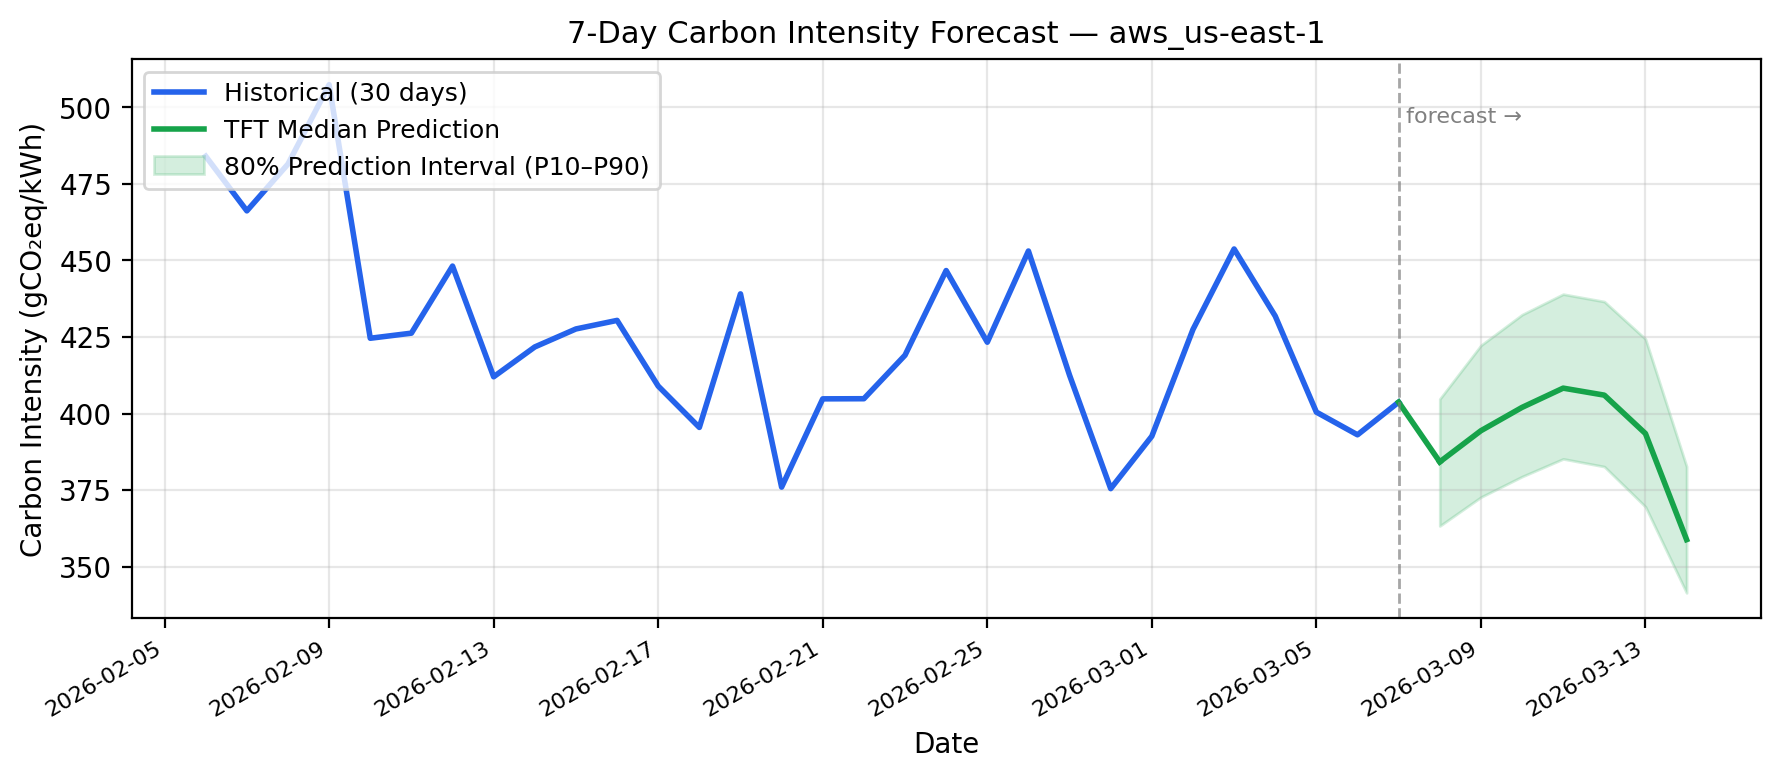
\includegraphics[width=0.72\textwidth]{figure_forecast}
\caption{Sample 7-day carbon intensity forecast for \texttt{aws\_us-east-1}. Solid line: 30-day historical data. Dashed line: TFT median prediction. Shaded area: 80\% prediction interval (P10--P90).}
\label{fig:forecast}
\end{figure}

\section{Discussion}

\subsection{Cost of Being Green}
The evaluation results demonstrate that the eco-optimized choice typically imposes a modest cost premium. In the example of Table~\ref{tab:pareto_results}, the eco-optimized instance costs 43\% more than the cheapest but achieves a 70\% reduction in carbon emissions. In practice, cost premiums for eco-optimized deployments typically range between 5--40\%, while emission reductions of 50--80\% are achievable. This trade-off is acceptable for organizations with sustainability commitments, particularly since cloud spend is only one dimension of total operational cost.

\subsection{Value of Forecasting}
TFT-based carbon intensity forecasting adds value beyond real-time optimization. Users planning batch jobs or flexible workloads 1--7 days in advance can leverage forecast trends to schedule computation in lower-emission windows. The probabilistic forecast intervals further enable risk-aware scheduling, allowing users to trade off between the most likely outcome and worst-case emission scenarios.

\subsection{Limitations and Scalability}
The fixed power parameters are approximations; actual consumption varies by processor generation and cooling efficiency. Carbon intensity is mapped at country level, which can obscure sub-regional grid variation (e.g., both \texttt{us-east-1} and \texttt{us-east-2} map to \texttt{US}). On-demand pricing is policy-driven and aperiodic, so the TFT targets only carbon intensity rather than cost. On the deployment side, the singleton forecaster serves cached forecasts with sub-millisecond latency, while pricing queries are bounded by external API response times (~1--3 seconds per provider); the system is designed for horizontal scalability.

\section{Conclusion and Future Work}
This paper presented CarbonEdge, an end-to-end multi-cloud optimization framework for cost- and carbon-aware decision-making. The system makes four primary contributions: (1) an interpretable instance-level carbon estimation model combining power estimation with real-time regional carbon intensity, (2) real-time multi-provider pricing integration across AWS, Azure, and GCP, (3) multi-objective Pareto analysis producing three actionable recommendations, and (4) a Temporal Fusion Transformer providing 7-day probabilistic carbon intensity forecasts across 60+ cloud regions.

Experimental evaluation demonstrates that region selection alone can cause more than a 12$\times$ difference in carbon emissions for identical workloads, and eco-optimized recommendations achieve 50--80\% emission reductions for modest cost premiums. CarbonEdge is deployed as a full-stack web application, making sustainability-aware cloud optimization accessible to practitioners without provider-level infrastructure access.

Future work includes extending coverage to GPU and serverless instances, incorporating spot pricing, integrating embodied carbon for lifecycle analysis, enabling sub-national grid mapping, and building automated scheduling agents that act on forecast trends to shift workloads to greener regions.

\section*{Acknowledgements}
The authors thank the Department of Computer Science and Engineering at PES University for academic guidance and project support. This work used publicly available resources, including the ElectricityMap API, AWS/Azure/GCP pricing resources, and open-source frameworks such as FastAPI, Next.js, PyTorch, and PyTorch Lightning.

\section*{Code Availability}
The open-source implementation of CarbonEdge is publicly available at: \url{https://github.com/Shah1011/CarbonEdge}.

\begin{thebibliography}{}
\small

\bibitem[Amazon Web Services(2025)]{b2} Amazon Web Services, ``AWS Customer Carbon Footprint Tool,'' \url{https://aws.amazon.com/aws-cost-management/aws-customer-carbon-footprint-tool/}, accessed Mar.\ 2025.

\bibitem[Dayarathna et~al.(2016)]{b11} M.~Dayarathna, Y.~Wen, and R.~Fan, ``Data center energy consumption modeling: A survey,'' \textit{IEEE Commun.\ Surveys Tuts.}, vol.\ 18, no.\ 1, pp.\ 732--794, 2016.

\bibitem[Deb et~al.(2002)]{b13} K.~Deb, A.~Pratap, S.~Agarwal, and T.~Meyarivan, ``A fast and elitist multiobjective genetic algorithm: NSGA-II,'' \textit{IEEE Trans.\ Evol.\ Comput.}, vol.\ 6, no.\ 2, pp.\ 182--197, Apr.\ 2002.

\bibitem[Dosanapudi et~al.(2025)]{b17} U.~K.~Dosanapudi, S.~Mohanty, and P.~K.~Pattnaik, ``Optimizing cloud costs and carbon footprint in multi-cloud environments with fuzzy logic \& Monte Carlo simulation,'' \textit{Journal of Theoretical and Applied Information Technology}, vol.\ 103, no.\ 16, 2025.

\bibitem[Garg et~al.(2013)]{b14} S.~K.~Garg, S.~Versteeg, and R.~Buyya, ``A framework for ranking of cloud computing services,'' \textit{Future Gener.\ Comput.\ Syst.}, vol.\ 29, no.\ 4, pp.\ 1012--1023, 2013.

\bibitem[Gartner(2024)]{b1} Gartner, ``Gartner forecasts worldwide public cloud end-user spending to surpass \$800 billion in 2025,'' Gartner Research, 2024.

\bibitem[Herzen et~al.(2022)]{b16} N.~Herzen et al., ``Darts: User-friendly modern machine learning for time series,'' \textit{J.\ Mach.\ Learn.\ Res.}, vol.\ 23, no.\ 124, pp.\ 1--6, 2022.

\bibitem[Khurana et~al.(2025)]{b18} R.~Khurana, A.~Kaur, and K.~Kaur, ``Comparative evaluation of cloud pricing models: Insights from AWS, Microsoft Azure, and GCP,'' \textit{International Journal of Scientific Research in Science and Technology}, vol.\ 12, no.\ 3, pp.\ 627--635, 2025.

\bibitem[Lim et~al.(2021)]{b15} B.~Lim, S.~\"{O}.~Ar{\i}k, N.~Loeff, and T.~Pfister, ``Temporal Fusion Transformers for interpretable multi-horizon time series forecasting,'' \textit{Int.\ J.\ Forecasting}, vol.\ 37, no.\ 4, pp.\ 1748--1764, 2021.

\bibitem[Microsoft(2025)]{b4} Microsoft, ``Microsoft Emissions Impact Dashboard,'' \url{https://www.microsoft.com/en-us/sustainability/emissions-impact-dashboard}, accessed Mar.\ 2025.

\bibitem[Pelley et~al.(2009)]{b10} S.~Pelley, D.~Meisner, T.~F.~Wenisch, and J.~W.~VanGilder, ``Understanding and abstracting total data center power,'' in \textit{Proc.\ Workshop on Energy-Efficient Design}, 2009, pp.\ 1--6.

\bibitem[Qi et~al.(2023)]{b19} S.~Qi, D.~Milojicic, C.~Bash, and S.~Pasricha, ``MOSAIC: A multi-objective optimization framework for sustainable datacenter management,'' in \textit{Proc.\ IEEE 30th Int.\ Conf.\ High Performance Computing, Data, and Analytics (HiPC)}, 2023, pp.\ 51--60.

\bibitem[Radovanovi\'{c} et~al.(2020)]{b3} A.~Radovanovi\'{c} et al., ``Carbon-intelligent computing for data centers,'' Google Research Blog, 2020.

\bibitem[Tomorrow(2025)]{b9} Tomorrow, ``ElectricityMap: Real-time CO\textsubscript{2} emissions of electricity consumption,'' \url{https://electricitymap.org}, accessed Mar.\ 2025.

\end{thebibliography}

\end{document}
